\documentclass[10pt]{article}

\usepackage[margin=0.76in]{geometry}
\usepackage[T1]{fontenc}
\usepackage[utf8]{inputenc}
\usepackage{lmodern}
\usepackage{microtype}
\usepackage{amsmath,amssymb}
\usepackage{booktabs}
\usepackage{tabularx}
\usepackage{array}
\usepackage{graphicx}
\usepackage{xcolor}
\usepackage{tikz}
\usetikzlibrary{arrows.meta,positioning}
\usepackage{caption}
\usepackage{float}
\usepackage{enumitem}
\usepackage{listings}
\usepackage{multicol}
\usepackage{titlesec}
\usepackage[hidelinks]{hyperref}

\captionsetup{font=small,labelfont=bf,skip=3pt}
\setlength{\parindent}{0pt}
\setlength{\parskip}{0.28em}
\setlength{\columnsep}{0.45cm}
\renewcommand{\arraystretch}{1.06}
\newcolumntype{Y}{>{\raggedright\arraybackslash}X}
\raggedbottom

\titleformat{\section}{\large\bfseries}{\thesection}{0.55em}{}
\titleformat{\subsection}{\normalsize\bfseries}{\thesubsection}{0.50em}{}
\titleformat{\subsubsection}{\normalsize\itshape}{\thesubsubsection}{0.45em}{}
\titleformat{\paragraph}[block]{\normalsize\itshape}{\theparagraph}{0.45em}{}
\titlespacing*{\section}{0pt}{0.55em}{0.25em}
\titlespacing*{\subsection}{0pt}{0.40em}{0.18em}
\titlespacing*{\subsubsection}{0pt}{0.30em}{0.12em}
\titlespacing*{\paragraph}{0pt}{0.30em}{0.12em}
\setcounter{secnumdepth}{4}

\definecolor{codebg}{RGB}{247,247,247}
\definecolor{codeframe}{RGB}{180,180,180}
\lstset{
  basicstyle=\ttfamily\footnotesize,
  columns=fullflexible,
  frame=single,
  rulecolor=\color{codeframe},
  backgroundcolor=\color{codebg},
  xleftmargin=0.22em,
  xrightmargin=0.22em,
  aboveskip=0.28em,
  belowskip=0.28em,
  showstringspaces=false,
  breaklines=true
}

\newcommand{\figureplaceholder}[3]{%
  \begin{figure}[H]
    \centering
    \fbox{\parbox[c][#1][c]{0.93\linewidth}{\small\raggedright
      \textbf{Image placeholder.} #2}}
    \caption{#3}
  \end{figure}%
}

\begin{document}
\begin{center}
  {\LARGE\bfseries Routly Planner: Scalable PDDL+ Urban Routing\par}
  \vspace{0.20em}
  {\large Model simplification, step-by-step replanning, and LLM road events\par}
  \vspace{0.65em}
  {\normalsize Cozza S. -- Cristiano F. -- Ielpa E. -- Rudi G.\par}
  \vspace{0.45em}
  {\normalsize \today\par}
\end{center}
\vspace{-0.35em}

\begin{abstract}
Routly Planner is a framework for urban route planning over real OpenStreetMap networks. It downloads a city's road map from OpenStreetMap with OSMnx, ENHSP solves a PDDL-based problem, and SUMO validates the resulting route in a traffic simulation. The model can include traffic that slows roads down, traffic lights, closed roads, and (optionally) fuel limits. These features make the routes more realistic, but they also increase the computational cost of planning. Routly studies two different scalability strategies. The \emph{model-side} branch improves scalability by simplifying the planning model before it is given to the planner. The \emph{controller-side} branch keeps the
detailed PDDL+ process model but solves the trip in smaller pieces and joins them, for congestion or for fuel. A separate LLM layer generates structured road closures and slowdowns using topology and start/goal information, without ever seeing the planned route; a second planning run then measures how well the route adapts. All modelling choices and experimental parameters are recorded through validated YAML configuration snapshots.
\end{abstract}
\vspace{-0.35em}

\section{Problem Description}

Routly receives a directed road graph $G=(L,R)$, where $L$ are locations (nodes) and $R$ are the roads connecting
them (edges). It also receives a vehicle $v$, a start location $s$, and a goal location
$g$. The task is to find a route that minimises a numeric cost while
respecting road availability and optional time and fuel constraints.

The current case study uses the drivable network of Bologna, Italy. OSMnx
downloads the network from OpenStreetMap and removes extra geometry-only points while
keeping real junctions, dead ends, road connections and road shapes
\cite{boeing2017,boeing2025}. Routly then crops the map to a chosen radius (\texttt{distance\_meters}), caps the number of nodes (\texttt{max\_nodes}), keeps only connected parts, and fixes a random seed so runs can be repeated.

Bologna is a good test case because its centre combines radial streets, a dense
secondary road network, and a ring structure \cite{nardino2021}. 

ENHSP chooses the route from the PDDL+ model. SUMO then simulates that route with background vehicles, used for visualization and validation \cite{lopez2018}.

\begin{figure}[H]
  \centering
  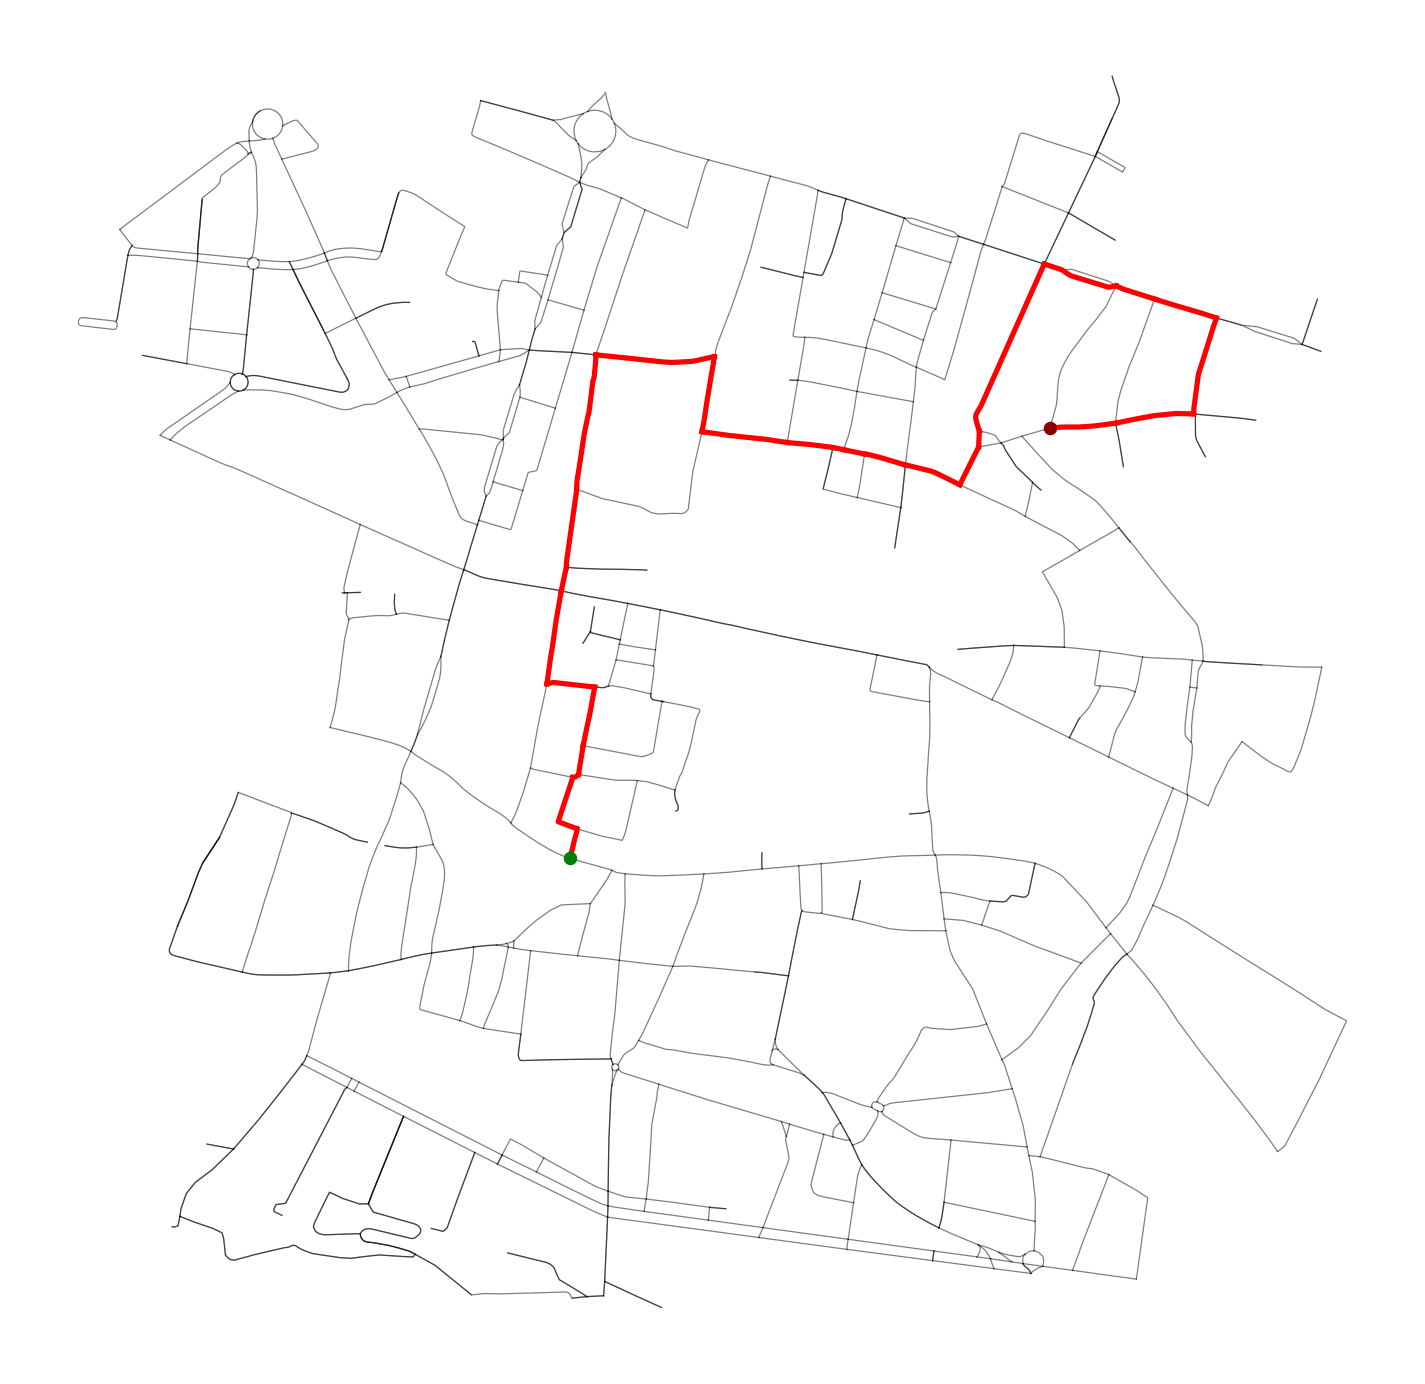
\includegraphics[width=0.40\linewidth]{images/basic_plan2goal.png}
  \caption{Visual PDDL planning result, from start node to goal node, over a map of the city of Bologna.}
  \label{fig:basic-plan-to-goal}
\end{figure}

\subsection{Why use PDDL+?}
Special graph algorithms such as Dijkstra, A*, and time-dependent routing are very good at finding shortest paths \cite{baum2015}, and they can even use traffic-based weights. Routly uses PDDL+ for a different reason: one planning model can
combine logical rules, numeric resources, time, and events. PDDL+ separates
agent actions, continuous processes, and events that happen automatically
\cite{foxlong2006}. This makes it suitable for describing movement,
fuel use, traffic-light delay, congestion, and road disruptions. Previous work already used PDDL+ for urban traffic control, especially for adjusting traffic-light
green phases \cite{vallati2016}. Routly instead studies the route of one vehicle
on a road network extracted automatically from a real city.

The biggest problem is scalability. More realistic features make the model
bigger. Numeric planning is strongly affected by the way the model is
written, and only a limited number of planners support rich PDDL+ models
\cite{scala2016,piotrowski2024}. Generic actions are especially costly when the
grounder receives many road, node, and time combinations, although most of them
are not valid road movements \cite{franco2019}.


\subsection{Research questions}
\begin{description}[leftmargin=1.05cm,labelwidth=0.85cm,itemsep=0.10em,topsep=0.05em]

  \item[\textbf{RQ1}] How much do the model-side optimisations improve planner scalability?

  \item[\textbf{RQ2}] Can the Python controllers solve larger routing problems by splitting them into smaller plans?

  \item[\textbf{RQ3}] Can the LLM generate useful road disruptions without seeing the original route?

\end{description}

\section{Modelling and Implementation}

\subsection{Realistic base domain}
\textbf{Traffic lights.} Signal nodes come from OSM. Each junction is labelled simple, medium, or complex from its number
of connected roads and the highest road class that reaches it. More complex
junctions receive longer green, yellow, and red phases. The planner uses an
expected red-light delay rather than predicting the exact light colour at
arrival:
\[
 d^{\mathrm{signal}}=\frac{r^2}{2(g+y+r)},
\]
where $g$, $y$, and $r$ are the green, yellow, and red durations. This follows
the standard idea of average signal delay \cite{webster1958}.

\begin{center}
\small
\begin{tabular}{@{}lccc@{}}
\toprule
Signal input & Level 0 & Level 1 & Level 2 \\
\midrule
Degree (roads meeting) & $\leq 2$ & $3$ & $\geq 4$ \\
Highest road class & local & arterial & major \\
\bottomrule
\end{tabular}
\qquad
\begin{tabular}{@{}lc@{}}
\toprule
Class & Score (degree + road) \\
\midrule
Simple & $0$ \\
Medium & $1$–$2$ \\
Complex & $3$–$4$ \\
\bottomrule
\end{tabular}
\end{center}

\textbf{Congestion.} Simulated background traffic represents the other
vehicles that create traffic load around the planned vehicle. Their routes are
used to count how many vehicles use each road. With the configured maximum
factor of 2.0, the implemented calculation can be written simply as
\[
 \text{congestion factor}
 =\min\!\left(2,\,1+\frac{\text{background vehicles on the road}}
                         {\text{saturation count for its road class}}\right).
\]
The saturation count reflects road capacity:

\begin{center}
\scriptsize
\begin{tabular}{@{}lccc@{}}
\toprule
Road class & Local & Arterial & Major \\
\midrule
Saturation count & 20 & 35 & 50 \\
\bottomrule
\end{tabular}
\end{center}

Congestion then affects route cost through two direct relationships:
\[
 \text{effective speed}=\frac{\text{speed limit}}{\text{congestion factor}},
 \qquad
 \text{road duration}=\frac{\text{road length}}{\text{effective speed}}
                       +\text{signal delay}.
\]
The signal delay is the expected traffic-light delay defined above and is zero
when the road does not end at a signal. In static mode, the factor and duration
remain fixed for the whole plan. In dynamic mode, Python computes one duration
per global window and writes it as \texttt{travel-duration-window}; a single
global event advances the active window for the network.

\begin{lstlisting}
;; Static congestion: fixed for the complete plan
(= (congestion-factor road_0001) 1.05)
(= (travel-duration road_0001) 12.40)

;; Dynamic congestion: one global sequence of windows
(= (sim-time) 0)
(current-window tw_00000)
(= (window-start tw_00000) 0)
(= (window-start tw_00030) 30)
(next-window tw_00000 tw_00030)

(= (travel-duration-window road_0002 tw_00000) 12.40)
(= (travel-duration-window road_0002 tw_00030) 18.10)

(:event advance-window
 :parameters (?from - time-window ?to - time-window)
 :precondition (and
   (current-window ?from)
   (next-window ?from ?to)
   (>= (sim-time) (window-start ?to)))
 :effect (and
   (not (current-window ?from))
   (current-window ?to)))
\end{lstlisting}

\textbf{Fuel} Fuel is a numeric resource. In discrete mode,
fuel is removed once for each road. In continuous mode, it decreases during the
PDDL+ movement process. Fuel stations can be read from OSM or sampled with a
fixed seed. The fuel
controller follows the general idea of planning routes together with refuelling
stops \cite{erdogan2012}.

\begin{lstlisting}
;; discrete 
(decrease (fuel-level ?v) (* (road-length ?r) (fuel-consumption-rate ?v)))

;; continuous (#t = time step)
(decrease (fuel-level ?v) (* #t (* (speed ?v) (fuel-consumption-rate ?v))))
\end{lstlisting}

\subsection{Model-side scalability}

All numerical examples use the same calibrated Bologna case. The input is
limited to 500 OSM nodes. Table~\ref{tab:size-reference} reports the target
model after the preprocessing steps described next. Here, $R$, $L$, and $W$
denote roads, locations, and time windows; $S$ and $D$ denote static and dynamic
roads. 

\begin{table}[H]
\centering
\caption{Fixed 500-node reference case used in the model-size examples.}
\label{tab:size-reference}
\scriptsize
\begin{tabular}{@{}ccccccc@{}}
\toprule
Input nodes & Roads $|R|$ & Locations $|L|$ & Windows $|W|$ & Static $S$ & Dynamic $D$ & Window length \\
\midrule
500 & 676 & 383 & 14 & 607 & 69 & 30 s \\
\bottomrule
\end{tabular}
\end{table}

\subsubsection{Hybrid congestion and macro-road abstraction}
The original congestion choices make either every road static or every road
dynamic. Hybrid congestion selects the representation road by road. Python
compares each road's congestion factors across all windows and applies
\[
 \max_w c_{r,w}-\min_w c_{r,w}\geq 0.10.
\]
A road remains dynamic only when its variation reaches this threshold.
Otherwise, it receives one static cost because keeping a separate value for
every window would add little information to the planner.

Macro-road abstraction is a separate preprocessing step. It merges linear road
chains before PDDL generation. Table~\ref{tab:macro-conditions} summarises the
conditions enforced while a chain grows. 

\begin{table}[H]
\centering
\caption{Conditions used to build a macro road.}
\label{tab:macro-conditions}
\scriptsize
\begin{tabularx}{\linewidth}{@{}>{\raggedright\arraybackslash}p{2.35cm}>{\raggedright\arraybackslash}Y>{\raggedright\arraybackslash}p{3.15cm}>{\raggedright\arraybackslash}p{2.15cm}@{}}
\toprule
Topology & Protected nodes & Road compatibility & Chain limits \\
\midrule
No branch, reversal, or cycle & Start, goal, traffic lights, fuel stations, and intersections & Same capacity class; speed difference at most 15\% & At most 8 segments and 1500 m \\
\bottomrule
\end{tabularx}
\end{table}

\begin{table}[H]
\centering
\caption{Effect of the two preliminary scalability improvements in the reference case.}
\label{tab:preliminary-size-effects}
\scriptsize
\begin{tabularx}{\linewidth}{@{}p{2.6cm}Y Y@{}}
\toprule
Improvement & Before & After \\
\midrule
Hybrid congestion & 676 dynamic roads; 9464 dynamic road-window values & 69 dynamic and 607 static roads; 966 dynamic road-window values \\
Macro roads & 702 roads; 393 locations & 676 roads; 383 locations \\
\bottomrule
\end{tabularx}
\end{table}

\begin{figure}[H]
  \centering
  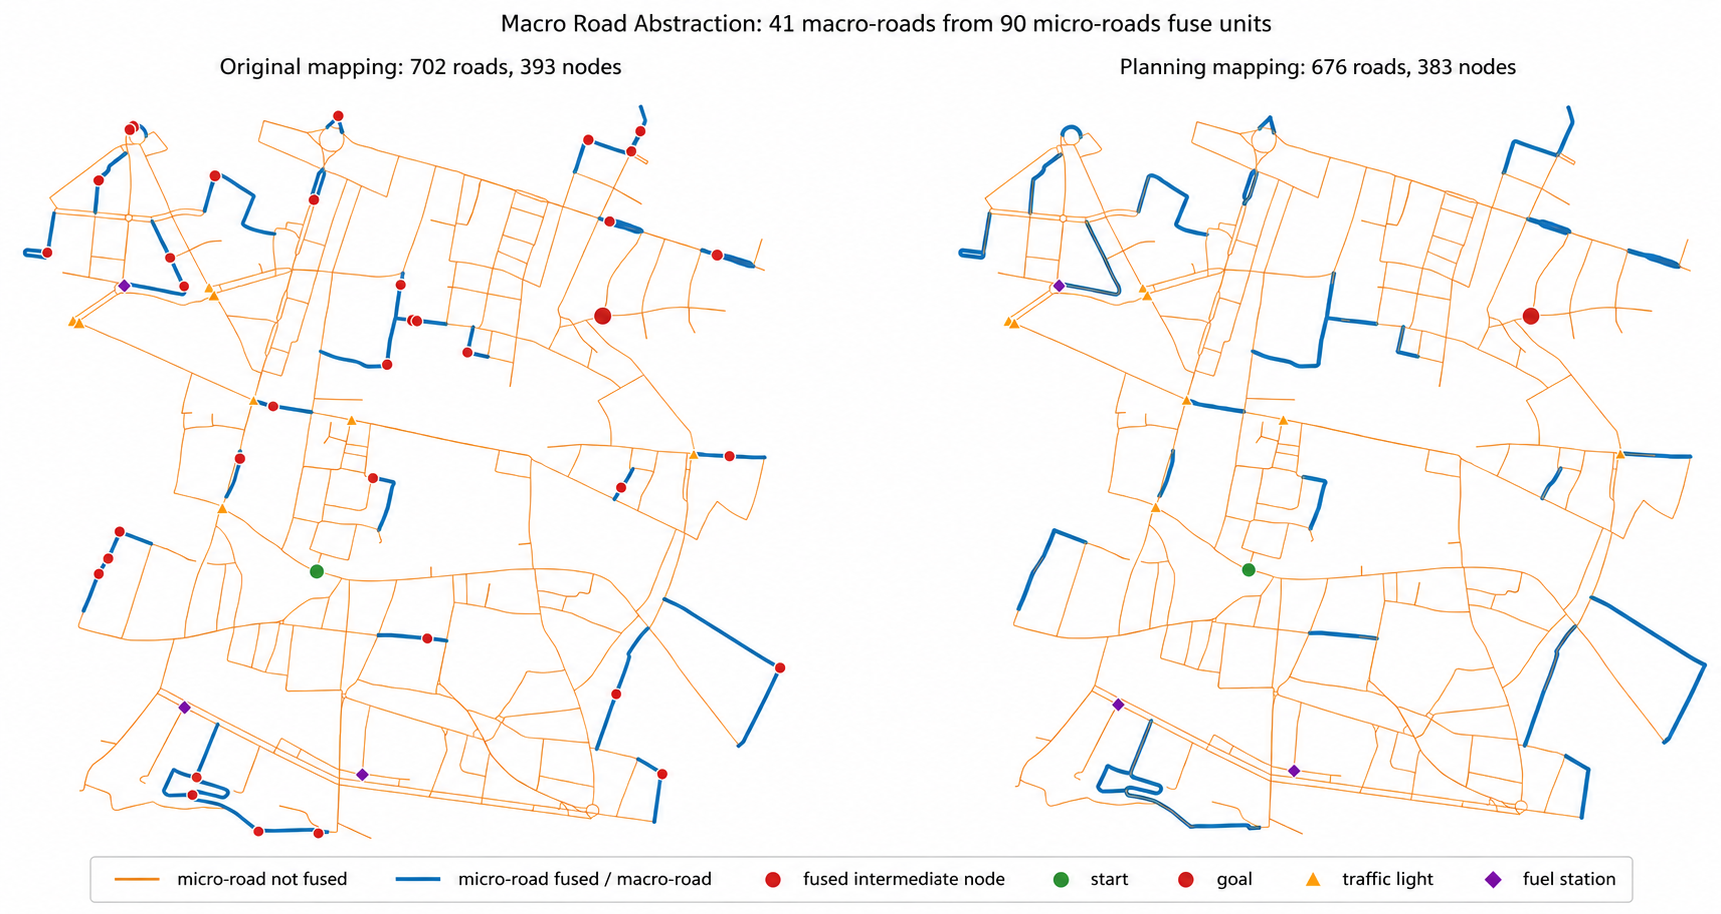
\includegraphics[width=0.90\linewidth]{images/macro_roads_comparison.png}
  \caption{Comparison between the original Bologna road network and its macro-road abstraction used before PDDL generation.}
  \label{fig:macro-roads-comparison}
\end{figure}

\subsubsection{Three modelling axes}
These two changes reduce the model before the main encoding choices are
applied. The larger model-side study then changes three independent axes,
summarised in Table~\ref{tab:model-axes} before the alternatives are discussed.

\begin{table}[H]
\centering
\caption{The three modelling axes used in the scalability study.}
\label{tab:model-axes}
\scriptsize
\begin{tabularx}{\linewidth}{@{}>{\raggedright\arraybackslash}p{2.35cm}>{\raggedright\arraybackslash}Y>{\raggedright\arraybackslash}p{3.15cm}@{}}
\toprule
Modelling axis & What it changes & Available choices \\
\midrule
Traversal model & How the vehicle crosses a road. & \texttt{process} or \texttt{compiled\_duration} \\
State representation & Whether the vehicle state is attached to a node or to an edge. & \texttt{node\_based} or \texttt{line\_graph} \\
Action generation & Whether action instantiation is handled by ENHSP or by Python. & \texttt{parameterized} or \texttt{compiled} \\
\bottomrule
\end{tabularx}
\end{table}

\paragraph{Process, node-based, parameterized baseline}
The baseline fixes the three axes as
\texttt{process + node\_based + parameterized}. The vehicle starts a road,
moves while the remaining distance decreases, and reaches the next node through
an arrival event. This is the only Routly variant that represents the vehicle
while it is on a road.

\begin{lstlisting}
(:action start-traversal
 :parameters (?v - vehicle ?r - road ?from ?to - location)
 :precondition (and (at ?v ?from) (connects ?r ?from ?to)
                    (road-open ?r) (not (moving ?v)))
 :effect (and (not (at ?v ?from)) (on-road ?v ?r) (moving ?v)
              (assign (distance-remaining ?v) (road-length ?r))))

(:process traverse
 :parameters (?v - vehicle)
 :precondition (and (moving ?v) (> (distance-remaining ?v) 0))
 :effect (decrease (distance-remaining ?v) (* #t (speed ?v))))

(:event arrive
 :parameters (?v - vehicle ?r - road ?from ?to - location)
 :precondition (and (on-road ?v ?r) (connects ?r ?from ?to) (<= (distance-remaining ?v) 0))
 :effect (and (not (moving ?v)) (not (on-road ?v ?r)) (at ?v ?to)))
\end{lstlisting}

The start and arrival schemas expose a road and its two endpoints. A dynamic
start action also contains a window parameter. The \texttt{connects} predicate
removes invalid combinations only after they have been handed to the grounder.

\begin{center}
\scriptsize
\begin{tabular}{@{}lll@{}}
\toprule
Reference formula & Substitution & Loose exposure \\
\midrule
$|R||L|^2(1+|W|)$ & $676\cdot383^2\cdot15$ & $1.487\times10^9$ assignments \\
\bottomrule
\end{tabular}
\end{center}

\paragraph{Compiled duration, node-based, parameterized}
The first change affects only the traversal axis. State representation remains
\texttt{node\_based} and action generation remains \texttt{parameterized},
giving \texttt{compiled\_duration + node\_based + parameterized}. Python
computes each duration from road length, speed, signal delay, and congestion;
one numeric PDDL action then moves the vehicle directly between two nodes.

\begin{lstlisting}
(:action traverse-road
 :parameters (?v - vehicle ?r - road ?from ?to - location)
 :precondition (and (at ?v ?from) (connects ?r ?from ?to)
                    (road-open ?r))
 :effect (and (not (at ?v ?from)) (at ?v ?to)
              (increase (travel-time ?v) (travel-duration ?r))))
\end{lstlisting}

This is a substantial semantic simplification even though it does not yet solve
grounding. In the core crossing encoding, three movement mechanisms become one,
the process and arrival event disappear, and no mid-road vehicle state must be
maintained. Table~\ref{tab:traversal-simplification} reports this structural
change separately from the grounding estimate.

\begin{table}[H]
\centering
\caption{Structural effect of compiling one road crossing into a numeric action.}
\label{tab:traversal-simplification}
\scriptsize
\begin{tabular}{@{}lcc@{}}
\toprule
Core encoding feature & Process baseline & Compiled duration \\
\midrule
Movement mechanisms & 3 (action + process + event) & 1 action \\
Autonomous mechanisms & 2 (process + event) & 0 \\
Mid-road vehicle fluents & 2 (remaining distance + speed) & 0 \\
Loose grounding exposure & $1.487\times10^9$ & $1.487\times10^9$ \\
\bottomrule
\end{tabular}
\end{table}

The generic action still exposes the road, source, destination, and window
parameters. Its dominant Cartesian product therefore remains the same as in
the process baseline.

\begin{center}
\scriptsize
\begin{tabular}{@{}lll@{}}
\toprule
Reference formula & Substitution & Loose exposure \\
\midrule
$|R||L|^2(1+|W|)$ & $676\cdot383^2\cdot15$ & $1.487\times10^9$ assignments \\
\bottomrule
\end{tabular}
\end{center}

\paragraph{Compiled duration, line graph, parameterized}
The traversal model remains \texttt{compiled\_duration} and action generation
remains \texttt{parameterized}; only the state representation changes. In
\texttt{compiled\_duration + line\_graph + parameterized}, the vehicle is ready
to traverse a road rather than located at a node. A generic action chooses the
current and next road, checks \texttt{(road-next ?r ?next)}, and replaces
\texttt{(ready-road ?v ?r)} with \texttt{(ready-road ?v ?next)}.

The node-based product over a road and two locations is replaced by a product
over the current road, its possible successor, and the window. Logical
filtering still occurs inside ENHSP, so invalid road pairs are still exposed to
the grounder.

\begin{center}
\scriptsize
\begin{tabular}{@{}lll@{}}
\toprule
Reference formula & Substitution & Loose exposure \\
\midrule
$|R|^2|W|$ & $676^2\cdot14$ & $6.40\times10^6$ assignments \\
\bottomrule
\end{tabular}
\end{center}

\paragraph{Compiled action generation with singleton types}
The final change moves action instantiation from ENHSP to Python. For every
valid transition, Python creates types that contain exactly one road, location,
or window object. The action keeps normal PDDL parameters, but each parameter
has only one type-compatible object. The following excerpt is taken from the
generated singleton encoding.

\begin{lstlisting}
(:types
 loc_type_loc_a loc_type_loc_b - location
 road_type_road_0001 - road)

(:objects
 loc_a - loc_type_loc_a
 loc_b - loc_type_loc_b
 road_0001 - road_type_road_0001)
\end{lstlisting}

The resulting action binds its road and endpoints to those singleton types:

\begin{lstlisting}
(:action traverse-road-static-road_0001
 :parameters (?v - vehicle ?r - road_type_road_0001
              ?from - loc_type_loc_a ?to - loc_type_loc_b)
 :precondition (and (at ?v ?from) (road-open ?r))
 :effect (and (not (at ?v ?from)) (at ?v ?to)
              (increase (travel-time ?v) (travel-duration ?r))))
\end{lstlisting}

This compilation can be applied to either state representation. For node-based
state, Python generates one schema for every static road and one for every
dynamic road-window pair. For line-graph state, $T_s$ and $T_d$ denote valid
static and dynamic road-to-road transitions; one additional schema completes
the goal road. This follows the wider idea that reformulating a planning model
can reduce grounding work \cite{franco2019}, and that temporal-numeric behaviour
can be compiled into a simpler form \cite{micheli2026}.

\begin{center}
\scriptsize
\begin{tabular}{@{}llll@{}}
\toprule
Compiled representation & Reference formula & Substitution & Generated schemas \\
\midrule
Node-based & $S+D|W|$ & $607+69\cdot14$ & $1573$ \\
Line graph & $T_s+T_d|W|+1$ & $1129+144\cdot14+1$ & $3146$ \\
\bottomrule
\end{tabular}
\end{center}

For this graph, compiled node-based action generation is the smallest final
encoding. The compiled line graph remains larger because one road can have
several valid successors, so road-to-road transitions outnumber roads.

\subsection{Controller-side scalability branch}
The second branch preserves the canonical
\texttt{process + node\_based + parameterized} model. Scalability is obtained
outside a single planner call: Python generates smaller problems, invokes
ENHSP repeatedly, executes a node-consistent prefix, updates global state, and
concatenates the partial plans. The two branches are complementary rather than
stacked: compiled traversal simplifies the model given to the planner, whereas
the controller retains the expressive process model and reduces the horizon of
each call.

\begin{figure}[H]
\centering
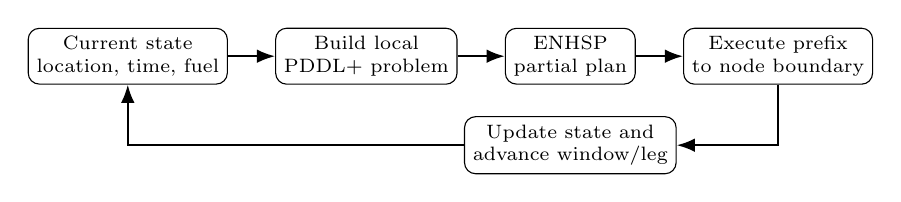
\begin{tikzpicture}[
  node distance=4mm and 6mm,
  box/.style={draw,rounded corners,align=center,minimum height=6mm,inner sep=3pt,font=\scriptsize},
  arr/.style={-Latex,thick}
]
\node[box] (state) {Current state\\location, time, fuel};
\node[box,right=of state] (problem) {Build local\\PDDL+ problem};
\node[box,right=of problem] (plan) {ENHSP\\partial plan};
\node[box,right=of plan] (prefix) {Execute prefix\\to node boundary};
\node[box,below=of plan] (update) {Update state and\\advance window/leg};
\draw[arr] (state) -- (problem);
\draw[arr] (problem) -- (plan);
\draw[arr] (plan) -- (prefix);
\draw[arr] (prefix.south) |- (update.east);
\draw[arr] (update.west) -| (state.south);
\end{tikzpicture}
\caption{Controller-side plan--execute-prefix--update loop.}
\label{fig:controller-loop}
\end{figure}

The \textbf{congestion controller} divides time into windows. For each window it
computes one static congestion snapshot, generates a process-model problem from
the current location to the unchanged final goal, and executes the last
completed traversal that fits the window. A node-boundary rule prevents the
next problem from inventing a location while the vehicle is still on a road. If the congestion factors on the unexecuted part of a cached plan are unchanged, the controller reuses it directly and skips that window's ENHSP call. Across iterations the congestion profile is dynamic, although each individual PDDL problem is static.

The \textbf{fuel controller} decomposes the route by reachability. If the final
goal is reachable with current fuel, it remains the planning target; otherwise
the controller selects a reachable fuel station according to its station
policy, solves that leg, updates fuel, and continues until the final goal is
reached. Fuel and congestion replanning are currently mutually exclusive.

\begin{figure}[H]
  \centering
  \begin{minipage}[t]{0.48\linewidth}
    \centering
    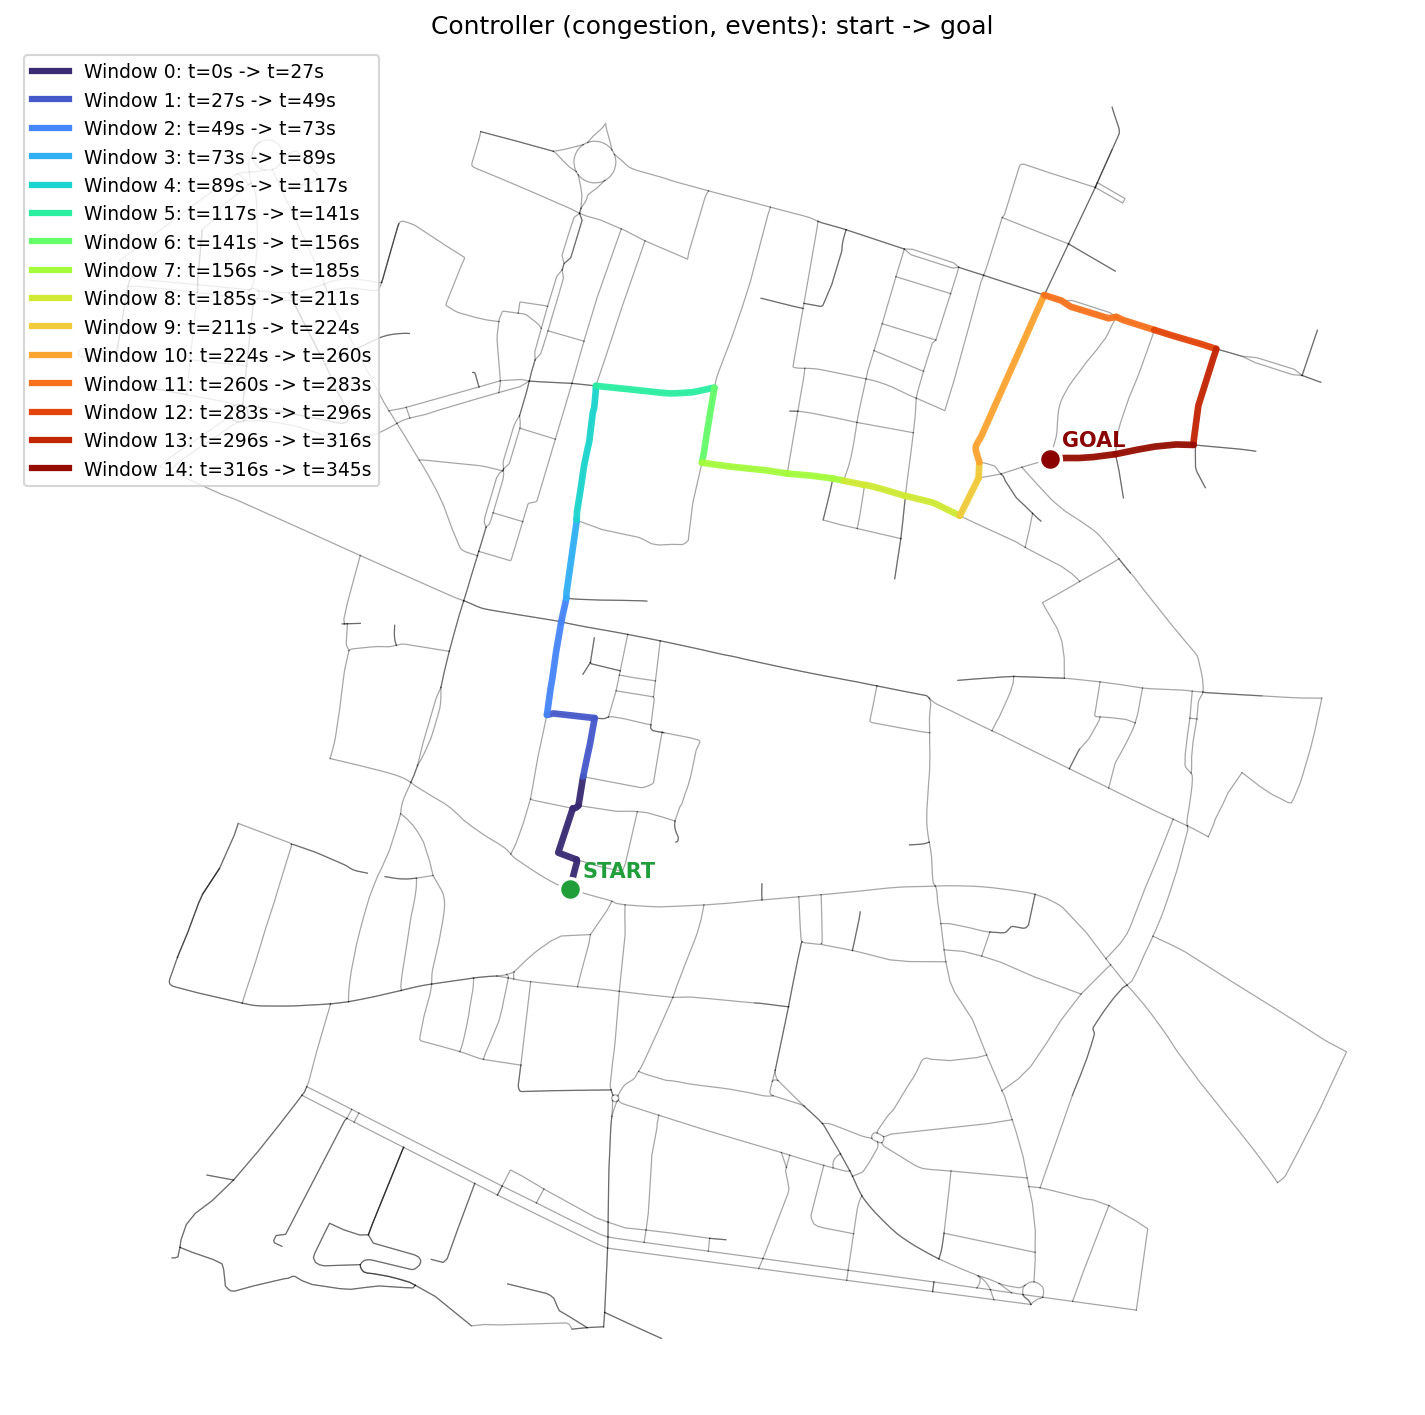
\includegraphics[width=\linewidth]{images/88_plan_dynamic_legs.png}
    \small (a) Congestion controller
  \end{minipage}\hfill
  \begin{minipage}[t]{0.48\linewidth}
    \centering
    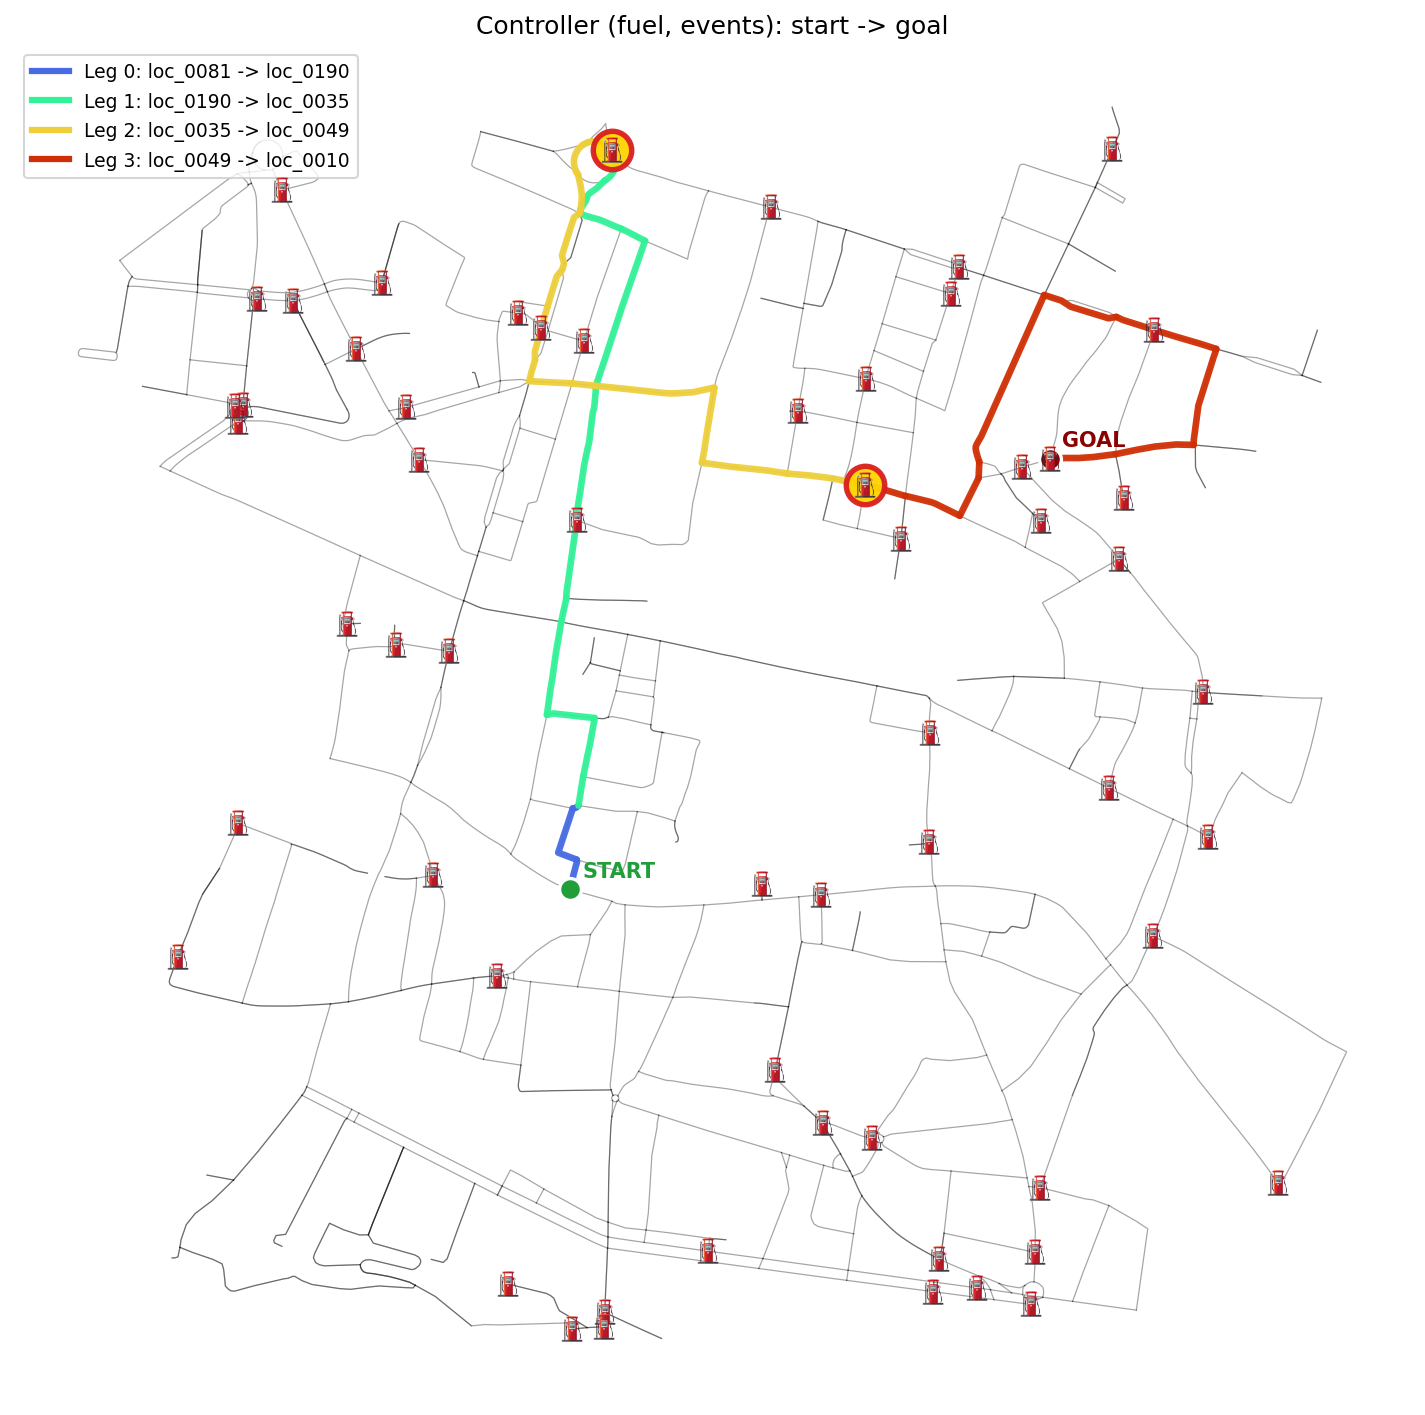
\includegraphics[width=\linewidth]{images/91_plan_dynamic_legs.png}
    \small (b) Fuel controller
  \end{minipage}
  \caption{Dynamic route decomposition into successive planning legs. The
  congestion controller (left) replans as traffic conditions change, whereas
  the fuel controller (right) selects reachable intermediate fuel stations.}
  \label{fig:dynamic-controller-legs}
\end{figure}

\section{Route-Unaware LLM Event Injection}



The LLM does not modify the PDDL domain directly. It generates a structured
event description, which is validated by Python and translated into a new PDDL
problem. Routly supports two closure patterns and one slowdown effect.

A \textbf{single-road closure} blocks one selected road. A
\textbf{multi-road closure} blocks a connected group of roads. When at least
two closed roads share the same intersection, that intersection is also
blocked. Start and goal locations are always protected.

The domain distinguishes the original availability of a road from a temporary
LLM disruption:

\begin{lstlisting}
(:predicates
  (road-open ?r - road)
  (road-blocked ?r - road)
  (location-blocked ?l - location)
)
\end{lstlisting}

The traversal action can use a road only when it is open and not affected by an
event.


A slowdown does not close the road. Instead, it increases its congestion
factor.

The roadmap is the following: 

\begin{figure}[H]
\centering
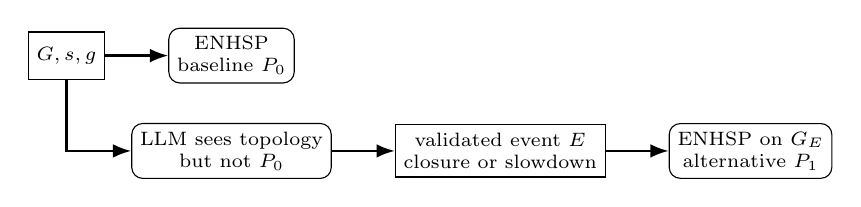
\begin{tikzpicture}[
  node distance=5mm and 8mm,
  box/.style={draw,rounded corners,align=center,minimum height=6mm,inner sep=3pt,font=\scriptsize},
  data/.style={draw,align=center,minimum height=6mm,inner sep=3pt,font=\scriptsize},
  arr/.style={-Latex,thick}
]
\node[data] (g) {$G,s,g$};
\node[box,right=of g] (p0) {ENHSP\\baseline $P_0$};
\node[box,below=of p0] (llm) {LLM sees topology\\but not $P_0$};
\node[data,right=of llm] (event) {validated event $E$\\closure or slowdown};
\node[box,right=of event] (p1) {ENHSP on $G_E$\\alternative $P_1$};
\draw[arr] (g) -- (p0);
\draw[arr] (g.south) |- (llm.west);
\draw[arr] (llm) -- (event);
\draw[arr] (event) -- (p1);
\end{tikzpicture}
\caption{Plan-hidden event generation and second planning run.}
\label{fig:llm-protocol}
\end{figure}


First, ENHSP produces a baseline plan
\[
  P_0=\operatorname{Plan}(G,s,g).
\]
The LLM then receives valid road identifiers, the incident nodes of each road,
$s$ and $g$, and optional geometric information, but it does not receive
$P_0$. It returns structured closures or slowdowns. A closure changes
\texttt{road-open}; a slowdown changes the congestion factor used to compute
travel duration. After schema and topology validation, the modified graph
$G_E$ is planned again from the same initial state:
\[
  P_1=\operatorname{Plan}(G_E,s,g).
\]

When the planning instance
contains at most 120 roads, both modes expose the complete road set to the LLM. When
\texttt{strategic\_injection=true}, Python instead selects at most 120 roads
from a geometric corridor around the straight start--goal segment and provides
each candidate's distance from that segment. 





\begin{figure}[H]
  \centering
  \includegraphics[width=0.65\linewidth]{images/500_nodes_event_map.png}
  \caption{Example on a 500-node network showing LLM events and
  the route found after the resulting closures and slowdowns.}
  \label{fig:500-nodes-event-map}
\end{figure}

\section{Results}
All comparisons use the same map seed, graph crop, start and goal, background
traffic, Java heap, ENHSP version, and feature settings. Each run stores the
resolved YAML, domain, problem, solver log, plan, event JSON, macro expansion,
and SUMO output.

\subsection{RQ1: model-side scalability}
Table~\ref{tab:rq1} reports the main verified grounding result on a Bologna case
with 677 roads, 384 locations, 14 windows, and an 8~GB Java heap. The generic
encoding exposed about $1.50\times10^9$ type-compatible assignments and ran out
of memory. The singleton model produced a complete plan.

\begin{table}[H]
\centering
\caption{Verified model-side result on the same 500-node case.}
\label{tab:rq1}
\scriptsize
\begin{tabularx}{\linewidth}{@{}p{2.4cm}Y p{1.45cm}p{3.25cm}@{}}
\toprule
Encoding & Symbolic exposure & Outcome & Measured evidence \\
\midrule
Generic parameterized & $677\cdot384^2\cdot(1+14)\approx1.50\times10^9$ assignments & Failed & Java out of memory after about 45.1~s; no plan. \\
Road-specific singleton & 427 static + 3500 dynamic schemas & Solved & Grounding 4.117~s; 3858 actions; 13 events; search 12.039~s; plan length 14. \\
Hybrid + macro roads & 607 static + 966 dynamic schemas & Solved & 69 dynamic roads; grounding 1.609~s; search 6.539~s; plan length 15. \\
\bottomrule
\end{tabularx}
\end{table}

The hybrid threshold is not universal. At $\theta=0.05$, 341 roads became
dynamic and runtime rose to about 20.7~s. At $\theta=0.10$, only 69 roads were
dynamic. Macro roads reduced the checked graph from 702 roads and 393 nodes to
676 roads and 383 nodes; 90 micro roads were grouped into 41 macro roads. The
reduction is modest because many urban intersections are real decision points.

\subsection{RQ2: controller-side scalability}
Table~\ref{tab:cong-controller} compares one full process-model solve with the
congestion controller. At 100 and 150 nodes, the controller greatly reduced
both grounding and planning time. At 1000 nodes, the full-horizon baseline did
not finish grounding, while the controller reached the goal through six real
planner calls and two cached windows.

\begin{table}[H]
\centering
\caption{Congestion controller using the same process model.}
\label{tab:cong-controller}
\scriptsize
\begin{tabular}{@{}r l r r r l@{}}
\toprule
Nodes & Mode & Calls & Grounding (s) & Planning (s) & Outcome \\
\midrule
100 & Full horizon & 1 & 270.0 & 494.2 & success, 204 steps \\
100 & Controller & 5 + 1 cached & 5.0 & 11.4 & success \\
150 & Full horizon & 1 & 821.2 & 3238.3 & success, 232 steps \\
150 & Controller & 5 + 2 cached & 21.5 & 48.5 & success \\
1000 & Full horizon & 1 & -- & -- & grounding did not finish \\
1000 & Controller & 6 + 2 cached & 947.2 & 2033.2 & success \\
\bottomrule
\end{tabular}
\end{table}

The fuel results show the same general pattern. The monolithic discrete and
continuous models solved only 100 and 150 nodes. From 200 nodes onward, both ran
out of memory. The fuel controller solved every tested size up to 1000 nodes,
although large cases could require many minutes. Traffic lights were enabled in
all runs.

\begin{table}[H]
\centering
\caption{Fuel experiments: total solver time in seconds. OOM means out of memory.}
\label{tab:fuel-results}
\scriptsize
\begin{tabular}{@{}r r r r@{}}
\toprule
Nodes & Monolithic discrete & Monolithic continuous & Fuel controller \\
\midrule
100  & 34.9 & 12.6 & 9.7 \\
150  & 58.2 & 116.3 & 31.7 \\
200  & OOM & OOM & 312.8 \\
300  & OOM & OOM & 327.9 \\
500  & OOM & OOM & 2769 \\
700  & OOM & OOM & 2665 \\
1000 & OOM & OOM & 847 \\
\bottomrule
\end{tabular}
\end{table}

The controller time is not monotonic because map shape, station position, and
the number of partial legs differ between instances. Its main benefit is that it
continues to produce a route when the single large problem cannot be grounded.

\subsection{RQ3: LLM event quality}
The current LLM study contains 35 strategic-injection runs over graph sizes from
100 to 1000 nodes. An event hit the hidden baseline route in 54.3\% of the runs.
Only 17.1\% of all runs changed the road sequence, because some hits changed the
cost without forcing a different route.

\begin{table}[H]
\centering
\caption{LLM event effect over 35 plan-hidden experiments.}
\label{tab:llm-results}
\scriptsize
\begin{tabularx}{\linewidth}{@{}Y r r Y@{}}
\toprule
Outcome & Count & Share & Average change in plan cost \\
\midrule
Event misses $P_0$ & 16 & 45.7\% & +1.0\% \\
Event hits $P_0$, same road sequence & 13 & 37.1\% & +12.8\% \\
Event hits $P_0$, route changes & 6 & 17.1\% & +12.9\%; mean Jaccard overlap $0.36$ \\
\bottomrule
\end{tabularx}
\end{table}

One 500-node example created a three-road closure cluster, one additional
accident closure, and a $2.8\times$ slowdown. Routly found a valid detour with
road-set overlap $J(P_0,P_1)=0.59$ and an 11.9\% cost increase. All reported
closures referred to real roads and remained solvable because the guard was
enabled. The +1.0\% average for missed events is not yet a clean zero because
background traffic was sometimes regenerated between $P_0$ and $P_1$. A final
controlled batch should freeze background traffic and include a guard-disabled
group to measure the true infeasibility rate.

\section{Code and Experimental Material}
All source code, configuration files, and experiments used to produce the
results reported in this paper are available in the Routly Planner GitHub
repository:
\href{https://github.com/GiuseppeRudi/routly-planner}{\texttt{github.com/GiuseppeRudi/routly-planner}}.

\section{Conclusions and Future Work}
Routly shows that the main limit of rich PDDL+ urban routing is the amount of detail and parameterisation given to the planner. The
model-side branch removes unnecessary mid-road state, generates only valid
road actions, uses singleton types, and applies time dependence only where it
matters. The controller-side branch keeps the detailed process model but spreads a whole route across smaller calls. The strongest verified result is the change
from an out-of-memory generic model to a complete singleton-typed plan on the
same 500-node case. The congestion and fuel controllers also solve larger cases
than their single-problem baselines. The LLM remains outside the route search
and creates checked, plan-hidden disruptions that test how well the route adapts.

The main future work is to combine the two controllers. Fuel should select the
next reachable target, congestion should set the costs for the current window,
ENHSP should choose the route, and Python should update location, time, fuel,
and refuelling before the next call. Other work includes online event injection
after part of the route has been driven, experiments on cities with different
road layouts, and a larger LLM study with fixed background traffic and the
solvability guard disabled in a separate test group.

\begin{multicols}{2}
\begin{thebibliography}{99}\scriptsize

\bibitem{foxlong2006}
M. Fox and D. Long, ``Modelling Mixed Discrete-Continuous Domains for
Planning,'' \emph{Journal of Artificial Intelligence Research}, vol. 27,
pp. 235--297, 2006. \url{https://doi.org/10.1613/jair.2044}

\bibitem{scala2016}
E. Scala, P. Haslum, S. Thi\'ebaux, and M. Ram\'irez, ``Interval-Based
Relaxation for General Numeric Planning,'' in \emph{Proc. ECAI}, pp. 655--663,
2016.

\bibitem{vallati2016}
M. Vallati, D. Magazzeni, B. De Schutter, L. Chrpa, and T. L. McCluskey,
``Efficient Macroscopic Urban Traffic Models for Reducing Congestion: A PDDL+
Planning Approach,'' in \emph{Proc. AAAI}, pp. 3188--3194, 2016.

\bibitem{franco2019}
S. Franco, M. Vallati, A. Lindsay, and T. L. McCluskey, ``Improving Planning
Performance in PDDL+ Domains via Automated Predicate Reformulation,'' in
\emph{Computational Science -- ICCS 2019}, pp. 491--498, 2019.

\bibitem{piotrowski2024}
W. Piotrowski and A. Perez, ``Real-World Planning with PDDL+ and Beyond,''
\emph{arXiv:2402.11901}, 2024.

\bibitem{micheli2026}
A. Micheli, E. Scala, and A. Valentini, ``Compiling Temporal Numeric Planning
into Discrete PDDL+: Extended Version,'' \emph{arXiv:2603.12188}, 2026.

\bibitem{baum2015}
M. Baum, J. Dibbelt, T. Pajor, and D. Wagner, ``Dynamic Time-Dependent Route
Planning in Road Networks with User Preferences,'' \emph{arXiv:1512.09132},
2015.

\bibitem{liu2023}
B. Liu, Y. Jiang, X. Zhang, Q. Liu, S. Zhang, J. Biswas, and P. Stone,
``LLM+P: Empowering Large Language Models with Optimal Planning Proficiency,''
\emph{arXiv:2304.11477}, 2023.

\bibitem{valmeekam2023}
K. Valmeekam, M. Marquez, S. Sreedharan, and S. Kambhampati, ``On the
Planning Abilities of Large Language Models: A Critical Investigation,''
\emph{arXiv:2305.15771}, 2023.

\bibitem{boeing2017}
G. Boeing, ``OSMnx: New Methods for Acquiring, Constructing, Analyzing, and
Visualizing Complex Street Networks,'' \emph{Computers, Environment and Urban
Systems}, vol. 65, pp. 126--139, 2017.

\bibitem{boeing2025}
G. Boeing, ``Modeling and Analyzing Urban Networks and Amenities with OSMnx,''
\emph{Geographical Analysis}, vol. 57, no. 4, pp. 567--577, 2025.

\bibitem{lopez2018}
P. Alvarez Lopez et al., ``Microscopic Traffic Simulation using SUMO,'' in
\emph{2018 IEEE Intelligent Transportation Systems Conference},
pp. 2575--2582, 2018.

\bibitem{nardino2021}
M. Nardino, L. Cremonini, T. Georgiadis, E. Mandanici, and G. Bitelli,
``Microclimate Classification of Bologna (Italy) as a Support Tool for Urban
Services and Regeneration,'' \emph{International Journal of Environmental
Research and Public Health}, vol. 18, no. 9, art. 4898, 2021.

\bibitem{webster1958}
F. V. Webster, \emph{Traffic Signal Settings}, Road Research Technical Paper
No. 39, HMSO, London, 1958.

\bibitem{erdogan2012}
S. Erdo\u{g}an and E. Miller-Hooks, ``A Green Vehicle Routing Problem,''
\emph{Transportation Research Part E}, vol. 48, no. 1, pp. 100--114, 2012.

\end{thebibliography}
\end{multicols}

\end{document}
